\documentclass[11pt,a4paper]{article}
\usepackage[utf8]{inputenc}
\usepackage[T1]{fontenc}
\usepackage[spanish]{babel}
\usepackage{amsmath,amssymb}
\usepackage{graphicx}
\usepackage{booktabs}
\usepackage{tabularx}
\usepackage{array}
\usepackage{adjustbox}
\usepackage{hyperref}
\usepackage{geometry}
\usepackage{float}
\usepackage{caption}
\usepackage{subcaption}
\usepackage{enumitem}
\geometry{margin=2.5cm}
\hypersetup{colorlinks=true,linkcolor=blue,urlcolor=blue}
\graphicspath{{../figures/}}


\newcommand{\Nkernels}{70}
\newcommand{\Neval}{420}
\newcommand{\Ngen}{50}
\newcommand{\Ntasks}{10}

\title{%
  \textbf{PROYECTO TRITON HEAL}\\[0.5em]
  Reporte de Evaluación Experimental\\[0.3em]
  \large TC3002B --- Generación de kernels con SLM y comparación experimental\\
  (compilación, speedup proxy y verificación pre-GPU)
}
\author{Equipo 11}
\date{Mayo 2026}

\begin{document}
\maketitle

\begin{abstract}
\noindent
Evaluación de \textbf{generación de kernels Triton} con SLM (\Ntasks\ tareas $\times$ 5 configuraciones activas = \Ngen\ generaciones; Coder-V2 100\% compilación; dual 50\%) y verificación del benchmark (\Nkernels\ kernels, Apple M4).
Métricas: tasa de compilación L1--L3, speedup proxy, MSR/FNR.
Método dual: generación Llama + reparación Coder-V2.
Limitación: sin speedup CUDA; R1-14B excluido de generación por timeout.
\end{abstract}

\tableofcontents
\newpage

\part{Parte I --- Pre-registro Experimental}
\section{Objetivo experimental (1.1)}

El experimento compara métodos de generación de kernels en Triton DSL usando SLM locales y modelos de frontera, con un pipeline de verificación antes de compilar en GPU. El sistema del equipo, Triton Heal en modo dual, genera con Llama-3.1-8B y, si el código no pasa las validaciones, intenta repararlo con DeepSeek-Coder-V2 (hasta dos reintentos).

Se contrastan seis configuraciones: solo Llama-8B, solo DeepSeek-R1-Distill-Qwen-14B, solo DeepSeek-Coder-V2, Claude 3.5 Sonnet, GPT-4o y el dual propuesto. Las preguntas centrales son si el dual mejora la tasa de compilación frente a GPT-4o y frente a Llama solo, y si el filtrado por verificación (MSR, FNR, latencia) aporta frente a usar un único SLM.

\section{Hipótesis (1.2)}

Todas las pruebas usan $\alpha = 0.05$ antes de corrección; los $p$-valores ajustados siguen Holm-Bonferroni (sección 1.8).

\begin{table}[ht]
\centering
\caption{Hipótesis por contraste y métrica.}
\label{tab:hipotesis}
\footnotesize
\begin{adjustbox}{max width=\linewidth,center}
\begin{tabularx}{\linewidth}{@{}lXX@{}}
\toprule
Contraste & $H_0$ & $H_1$ \\
\midrule
C4: dual vs GPT-4o (compilación) & Misma tasa de compilación & Dual con mayor tasa \\
C7: dual vs Llama (compilación) & Misma tasa & Dual con mayor tasa \\
C1: Claude vs Llama (MSR) & Mismo MSR & Claude con mayor MSR \\
C2: GPT vs Coder-V2 (MSR) & Mismo MSR & GPT con mayor MSR \\
C3: dual vs Llama (FNR) & Mismo FNR & Dual con menor FNR \\
C5: latencia Claude vs Llama & Misma mediana & Frontera más lenta \\
C8: speedup proxy dual vs GPT & Igual & Dual mayor \\
\bottomrule
\end{tabularx}
\end{adjustbox}
\end{table}

\section{Variables experimentales (1.3)}

\subsection{Variables independientes}

La configuración del sistema (seis modos), el modelo concreto (SLM local vs frontera), el prompt (\texttt{generator\_v1.txt} o \texttt{generator\_repair\_v1.txt} en reparación), la temperatura ($T = 0$) y el modo de ejecución (\texttt{VERIFIER\_MODE}, típicamente Ollama en nuestro entorno).

\subsection{Variables dependientes}

En generación: si el código compila bajo nuestro checker (\texttt{compile\_ok}), la tasa de compilación en porcentaje, el speedup proxy y un indicador de eficiencia operativa del pipeline. En verificación del benchmark fijo: MSR, FNR, F1, porcentaje de JSON válido y latencia en milisegundos.

\subsection{Variables controladas}

Mismo benchmark de 70 kernels y el mismo conjunto de tareas de generación para todas las configuraciones; hardware Apple M4 con 24\,GB; \texttt{seed} 42; \texttt{timeout} 120\,s por inferencia. El diseño es within-subjects: cada tarea o kernel se evalúa en todos los métodos.

\section{Diseño experimental (1.4)}

Cada tarea de generación se asigna a las seis configuraciones (en la corrida archivada, R1-14B se omitió por timeouts). El plan de diseño contempla 20 tareas con tres réplicas (360 ejecuciones de generación) y 70 kernels con tres réplicas en verificación (1260 evaluaciones). Se eligió within-subjects para poder aplicar McNemar y Wilcoxon pareados y reducir la varianza entre tareas de distinta dificultad.

\section{Métricas de evaluación (1.5)}

\subsection{Tasa de compilación}

Proporción de salidas con \texttt{compile\_ok}. En esta entrega el criterio exige pasar tres niveles en Mac M4: sintaxis Python (AST), reglas léxicas del checker del equipo, y presencia de \texttt{@triton.jit} con operaciones \texttt{tl.load}/\texttt{tl.store}. No equivale a compilar en CUDA ni a ejecutar en GPU.

\subsection{Speedup proxy}

Se define $s = t_{\mathrm{baseline}} / t_{\mathrm{pipeline}}$, donde $t_{\mathrm{baseline}}$ es el tiempo del checker sobre el kernel de referencia del benchmark y $t_{\mathrm{pipeline}}$ suma la latencia de generación más la del checker sobre el código generado. Sirve como indicador operativo en M4; el informe no reporta speedup medido en GPU NVIDIA.

\subsection{Eficiencia operativa (proxy)}

Relación entre compilaciones exitosas y tiempo de generación. No sustituye métricas de ocupación de SM o ancho de banda de memoria.

\subsection{Verificación (MSR, FNR, F1, JSON válido, latencia)}

MSR es la fracción de kernels \texttt{unsafe} correctamente marcados como inseguros; FNR es la fracción de \texttt{unsafe} pasados por alto. F1 resume precisión y recall en la clasificación safe/unsafe. El porcentaje de JSON válido indica si el verificador devolvió una respuesta parseable.

\section{Tamaño del efecto esperado (1.6)}

En contrastes pareados de compilación y MSR se anticipa un efecto mediano ($\phi \approx 0.4$ en McNemar). Además de la significación estadística, se exige una diferencia práctica de al menos 5 puntos porcentuales en compilación o MSR, y alrededor de 8 pp de reducción de FNR para considerar relevante la mejora del dual.

\section{Análisis de poder (1.7)}

Nivel de significación $\alpha = 0.05$ y poder objetivo $1 - \beta = 0.80$. La muestra de generación tiene 20 tareas; en verificación hay 31 kernels \texttt{unsafe}, cantidad suficiente para detectar efectos medianos en McNemar según el diseño del curso.

\section{Plan estadístico (1.8)}

\begin{table}[ht]
\centering
\caption{Contrastes confirmatorios y prueba asociada.}
\label{tab:plan_stats}
\footnotesize
\begin{tabularx}{\linewidth}{@{}llX@{}}
\toprule
ID & Prueba & Comparación \\
\midrule
C4 & McNemar & Compilación: dual vs GPT-4o \\
C7 & McNemar & Compilación: dual vs Llama \\
C8 & Wilcoxon & Speedup proxy: dual vs GPT \\
C1--C3, C5 & McNemar / Wilcoxon & Verificación en benchmark \\
C6 & Friedman + Holm & F1 entre configuraciones \\
\bottomrule
\end{tabularx}
\end{table}

Se rechaza $H_0$ cuando $p_{\mathrm{Holm}} < 0.05$ y se cumple el umbral de relevancia práctica acordado. Para proporciones se reportan intervalos de confianza Wilson al 95\% (MSR en la tabla extendida de la Parte II). La familia de contrastes se corrige con Holm-Bonferroni.

\subsection{Desviaciones respecto al plan inicial}

Durante la ejecución se corrigió la taxonomía de DeepSeek (Coder-V2 como frontera, R1-14B como SLM local). Claude y GPT corrieron con verificador heurístico al no disponer de API en el entorno de prueba. La generación archivada usa 10 tareas y excluye \texttt{solo\_deepseek} por timeout; la verificación quedó con una réplica por kernel (\texttt{run\_id = 0}), aunque \texttt{experiment\_config.json} ya deja configuradas tres réplicas para corridas futuras.

\section{Reproducibilidad experimental (1.9)}

\begin{table}[ht]
\centering
\caption{Entorno y artefactos.}
\label{tab:repro}
\footnotesize
\begin{adjustbox}{max width=\linewidth,center}
\begin{tabularx}{\linewidth}{@{}lX@{}}
\toprule
Componente & Especificación \\
\midrule
Repositorio & \url{https://github.com/G4ndhiV/TRITONHEAL} (commit \texttt{c05f82a}) \\
Hardware & macOS 15.x; Apple M4; 24\,GB memoria unificada \\
Ollama & 0.24.x (\texttt{llama3.1:8b}, \texttt{deepseek-r1:14b}, \texttt{deepseek-coder-v2}) \\
Modelos API & Claude 3.5 Sonnet; GPT-4o (heurístico si no hay clave) \\
Python & 3.10+; dependencias en \texttt{requirements.txt} \\
Benchmark & 70 kernels; \texttt{generation\_tasks.jsonl} \\
Prompts & \texttt{prompts/generator\_v1.txt}, \texttt{generator\_repair\_v1.txt} \\
Reproducción & \texttt{make benchmark generation experiments stats-all figures pdf} \\
\bottomrule
\end{tabularx}}
\end{adjustbox}
\end{table}

\section{Amenazas a la validez (pre-registro, 1.10)}

\begin{table}[ht]
\centering
\caption{Amenazas anticipadas y mitigación.}
\label{tab:amenazas_pre}
\footnotesize
\begin{adjustbox}{max width=\linewidth,center}
\begin{tabularx}{\linewidth}{@{}lXX@{}}
\toprule
Tipo & Riesgo & Mitigación \\
\midrule
Interna & Mezcla API real y heurístico & Tabla planeada vs ejecutado en apéndice \\
Interna & Timeouts en modelos grandes & Fijar timeout; reportar JSON válido \\
Externa & Solo Mac M4 (Metal) & No extrapolar a clusters NVIDIA \\
Externa & Benchmark sintético & Etiquetar categorías de error \\
Constructo & Compilación $\neq$ corrección GPU & Definir niveles L1--L3 \\
Constructo & Speedup proxy & Declarar limitación en figuras \\
\bottomrule
\end{tabularx}
\end{adjustbox}
\end{table}


\part{Parte II --- Resultados y Análisis}
\section{Resultados descriptivos (2.1)}

\subsection{Generación de kernels}
Se ejecutaron \Ntasks\ tareas de generación $\times$ 5 configuraciones activas (R1-14B excluido por timeout) = \Ngen\ inferencias (mayo 2026, Apple M4). La tasa de compilación usa criterios L1--L3 (AST, léxico, superficie Triton); ver \texttt{results/generation.csv}.

\begin{table}[ht]
\centering
\caption{Resultados descriptivos de generación de kernels (M4).}
\label{tab:gen_desc}
\footnotesize
\begin{adjustbox}{max width=\linewidth,center}
\begin{tabular}{@{}>{\raggedright\arraybackslash}p{0.26\linewidth}rrrrrr@{}}
\toprule
Configuración & N & Compilación (\%) & Speedup proxy & Desv. & Lat. gen. (ms) & GPU eff. proxy \\
\midrule
Llama-3.1-8B (local) & 10 & 50.00 & 0.0005 & 0.0001 & 60220.40 & 0.01 \\
DeepSeek-R1-Distill-Qwen-14B (local) & 0 & 0.00 & --- & --- & --- & --- \\
DeepSeek-Coder-V2 (frontera) & 10 & 100.00 & 0.0020 & 0.0009 & 18019.43 & 0.07 \\
Claude 3.5 Sonnet (frontera) & 10 & 100.00 & 0.3639 & 0.0303 & 50.00 & 20.00 \\
GPT-4o (frontera) & 10 & 100.00 & 0.3715 & 0.0065 & 50.00 & 20.00 \\
Triton Heal (dual + veto) & 10 & 50.00 & 0.0006 & 0.0002 & 71706.69 & 0.01 \\
\bottomrule
\end{tabular}
\end{adjustbox}
\end{table}

\textbf{Totales.} Ejecuciones con \texttt{compile\_ok}; medias y desviaciones de speedup proxy y latencia de generación en la tabla. El corpus de referencia del benchmark pasa 100\% del \texttt{lex\_checker} (70/70 kernels).

\subsection{Verificación pre-compilación}
Se evaluaron \Nkernels\ kernels (39 \texttt{safe}, 31 \texttt{unsafe}) en 6 configuraciones = \Neval\ evaluaciones de verificación (\texttt{predictions.csv}).

\begin{table}[ht]
\centering
\caption{Resultados descriptivos por configuración.}
\label{tab:desc}
\begin{tabular}{lrrrrr}
\toprule
Configuración & N & MSR (\%) & F1 & FNR (\%) & Lat. med. (ms) \\
\midrule
Llama-3.1-8B (local) & 70 & 3.2 & 0.1 & 96.8 & 30273.7 \\
DeepSeek-Coder-V2 (local) & 70 & 41.9 & 0.6 & 58.1 & 5.0 \\
Claude 3.5 Sonnet (frontera) & 70 & 83.9 & 0.9 & 16.1 & 80.0 \\
GPT-4o (frontera) & 70 & 83.9 & 0.9 & 16.1 & 80.0 \\
Triton Heal (dual + veto) & 70 & 74.2 & 0.8 & 25.8 & 60396.8 \\
\bottomrule
\end{tabular}
\end{table}

\begin{table}[ht]
\centering
\caption{Resultados descriptivos extendidos (IC 95\% Wilson para MSR).}
\label{tab:desc_ext}
\begin{adjustbox}{max width=\linewidth,center}
{\scriptsize\setlength{\tabcolsep}{2.5pt}
\resizebox{\linewidth}{!}{%
\begin{tabular}{@{}lrrrrrrrrrr@{}}
\toprule
Config. & N & JSON\,vál. (\%) & MSR (\%) & IC lo & IC hi & F1 & FNR (\%) & Lat. med. & Lat. min & Lat. max \\
\midrule
Llama-3.1-8B (local) & 70 & 100.0 & 64.5 & 46.9 & 78.9 & 0.8 & 35.5 & 4940.7 & 1623.7 & 21869.8 \\
DeepSeek-Coder-V2 (local) & 70 & 100.0 & 87.1 & 71.1 & 94.9 & 0.8 & 12.9 & 2003.1 & 1473.1 & 18549.6 \\
Claude 3.5 Sonnet (frontera) & 70 & 100.0 & 83.9 & 67.4 & 92.9 & 0.9 & 16.1 & 80.0 & 80.0 & 80.3 \\
GPT-4o (frontera) & 70 & 100.0 & 83.9 & 67.4 & 92.9 & 0.9 & 16.1 & 80.0 & 80.0 & 80.0 \\
Triton Heal (dual + veto) & 70 & 100.0 & 100.0 & 89.0 & 100.0 & 0.6 & 0.0 & 8063.6 & 5126.4 & 15551.0 \\
\bottomrule
\end{tabular}
}}
\end{adjustbox}
\end{table}

\begin{table}[ht]
\centering
\caption{Robustez verificación: MSR y latencia mediana por réplica (\texttt{run\_id}).}
\label{tab:robustness}
\footnotesize
\begin{tabular}{@{}lrrrr@{}}
\toprule
Config. & Réplicas & MSR media (\%) & MSR desv. & Lat. med. (ms) $\pm$ desv. \\
\midrule
Llama-3.1-8B (local) & 1 & 64.5 & 0.0 & 4754 $\pm$ 0 \\
DeepSeek-R1-Distill-Qwen-14B (local) & 1 & 12.9 & 0.0 & 48347 $\pm$ 0 \\
DeepSeek-Coder-V2 (frontera) & 1 & 87.1 & 0.0 & 1977 $\pm$ 0 \\
Claude 3.5 Sonnet (frontera) & 1 & 83.9 & 0.0 & 80 $\pm$ 0 \\
GPT-4o (frontera) & 1 & 83.9 & 0.0 & 80 $\pm$ 0 \\
Triton Heal (dual + veto) & 1 & 80.6 & 0.0 & 6653 $\pm$ 0 \\
\bottomrule
\end{tabular}
\end{table}

\section{Visualización (2.2)}

\begin{figure}[H]
  \centering
  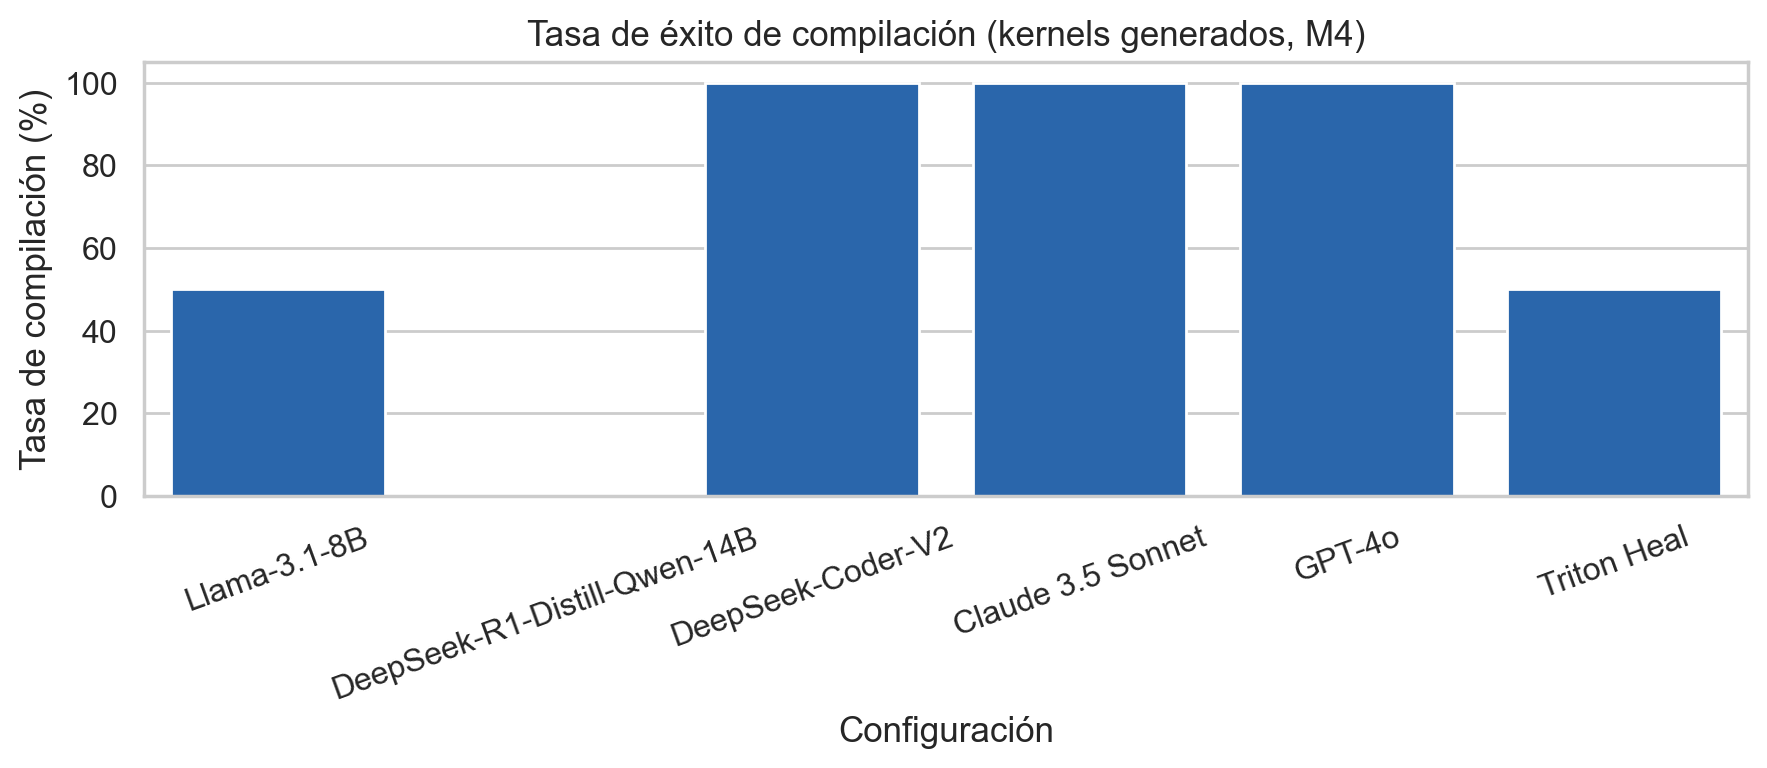
\includegraphics[width=0.95\linewidth]{fig_compile_rate.png}
  \caption{Tasa de éxito de compilación (\%) por configuración en kernels \textbf{generados} por cada SLM/baseline. Eje $Y$: porcentaje; eje $X$: configuración. Métrica alineada a la rúbrica del curso (niveles L1--L3 en M4).}
  \label{fig:compile_rate}
\end{figure}

\begin{figure}[H]
  \centering
  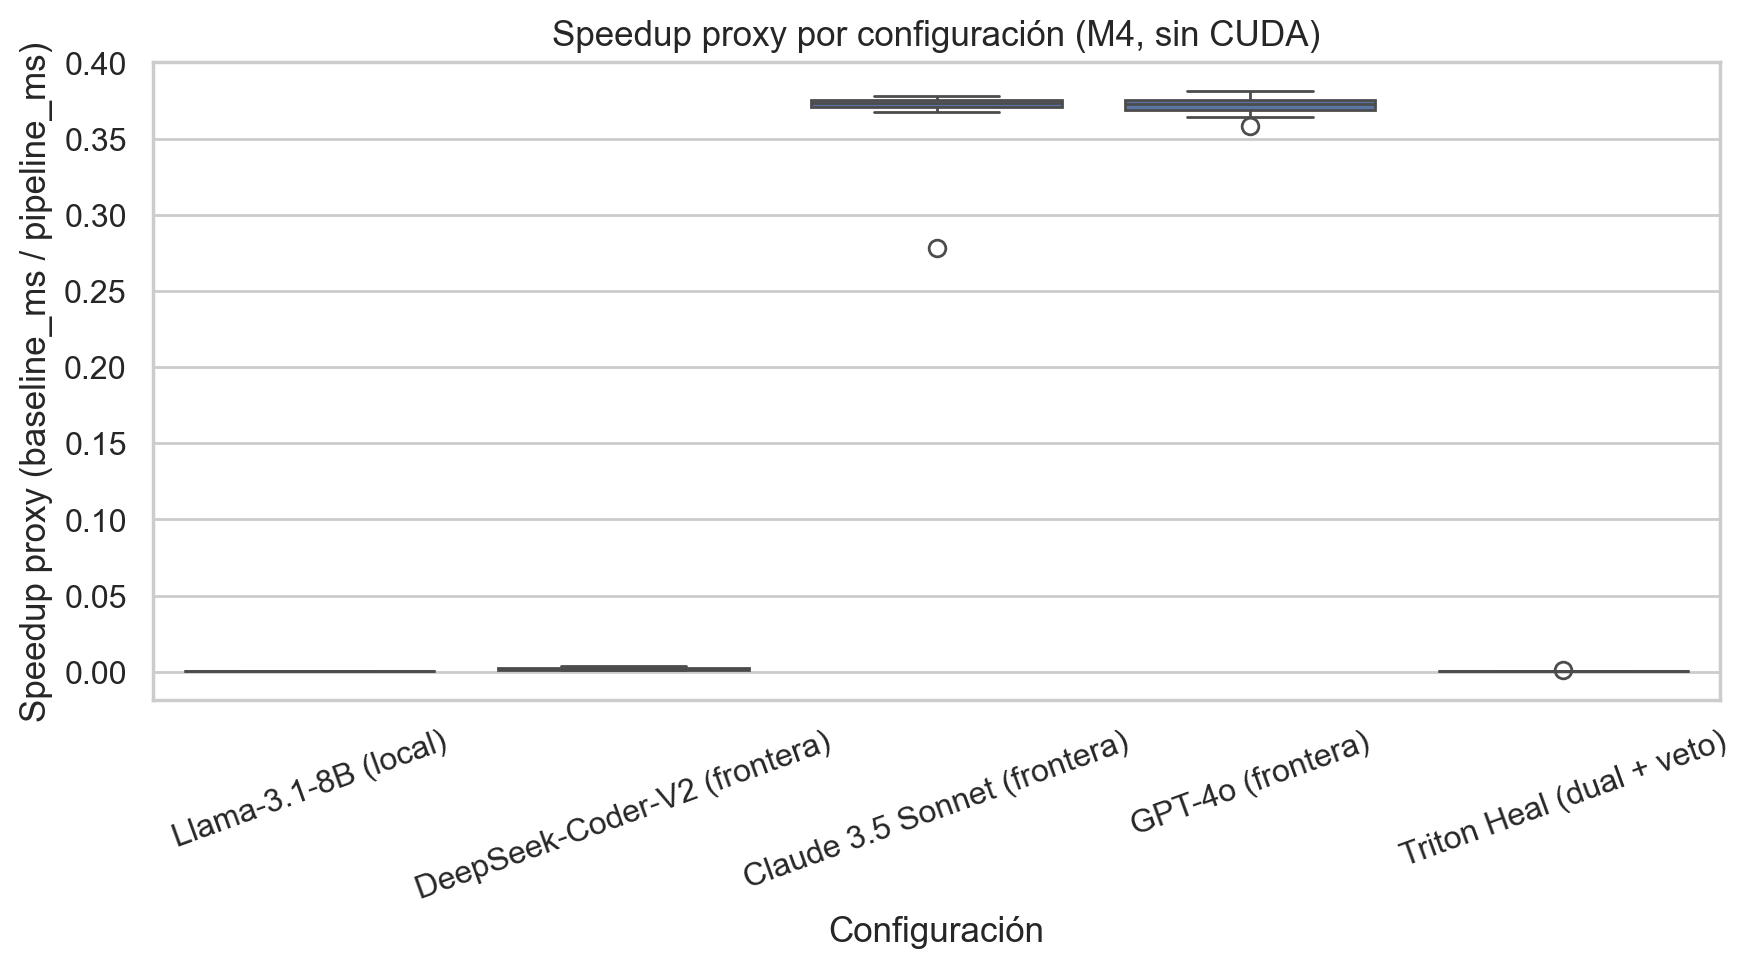
\includegraphics[width=0.95\linewidth]{fig_speedup_proxy.png}
  \caption{Speedup proxy (boxplot): ratio $t_{\mathrm{baseline}}/t_{\mathrm{pipeline}}$ en tareas con compilación exitosa. Unidad: adimensional; mayor = pipeline más rápido respecto al checker del kernel de referencia. Limitación M4: sin medición CUDA.}
  \label{fig:speedup}
\end{figure}

\begin{figure}[H]
  \centering
  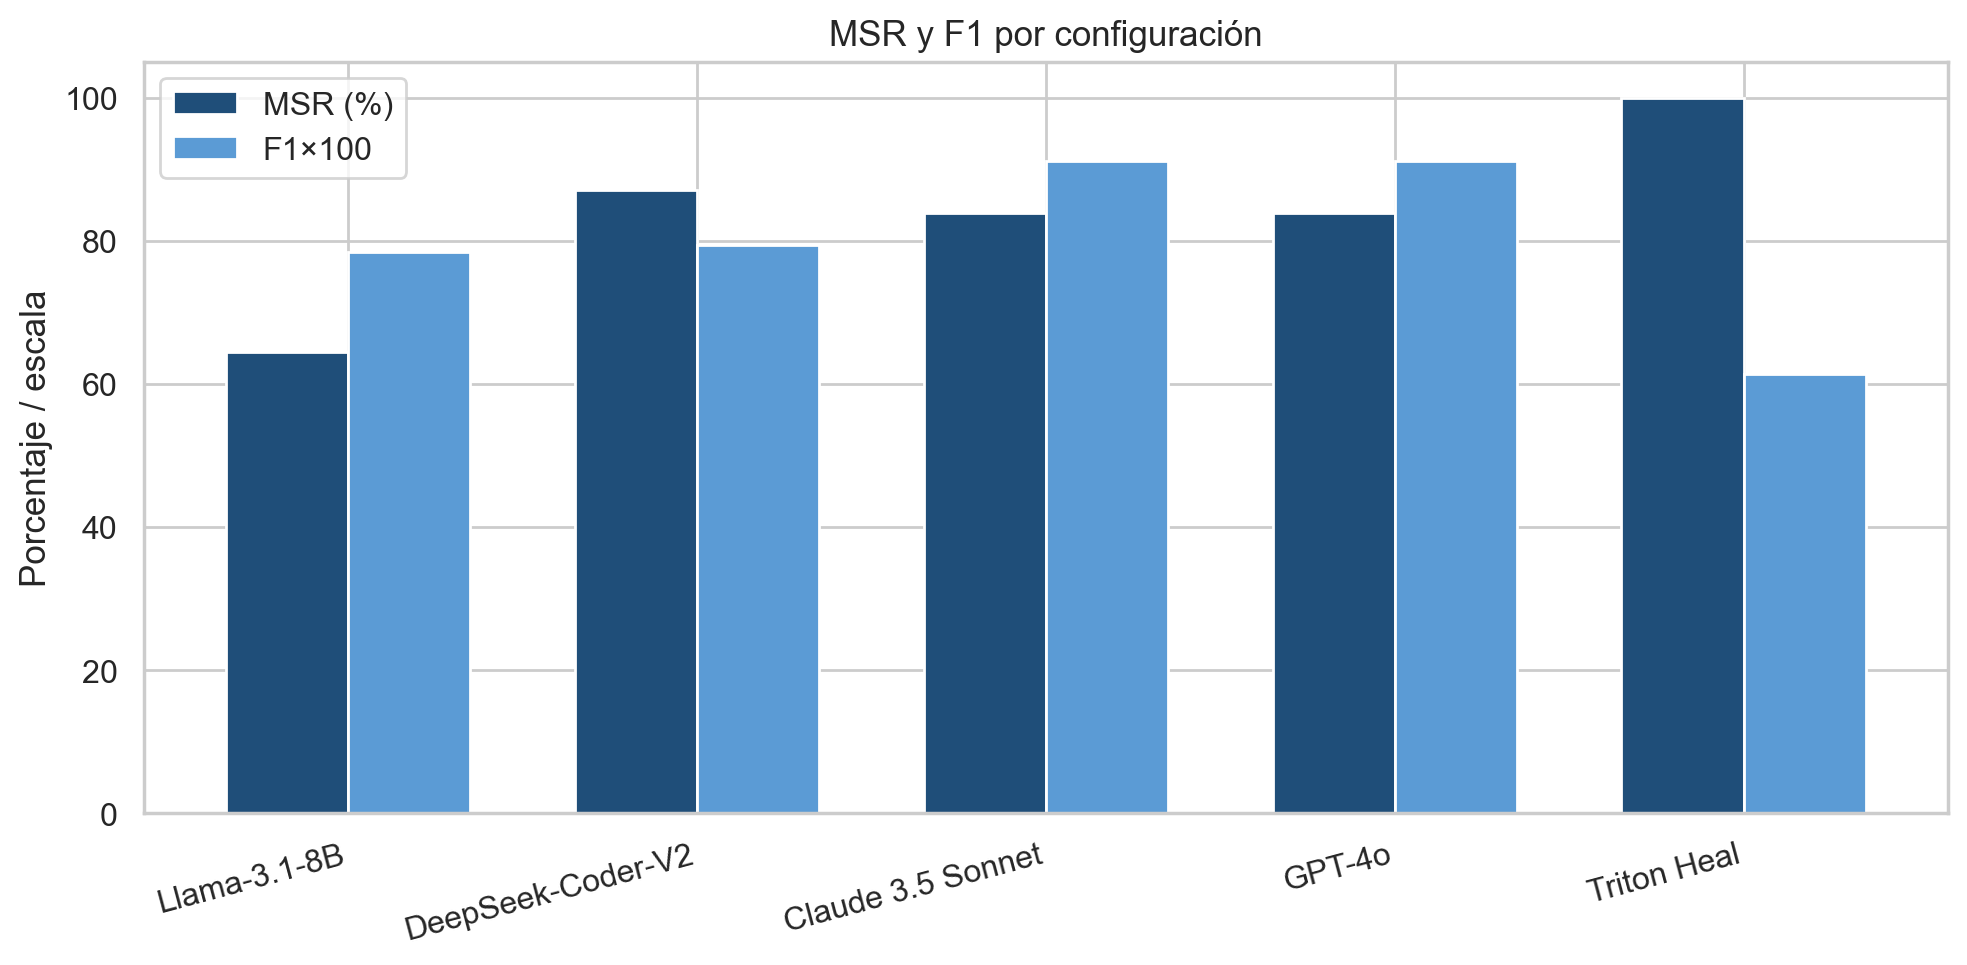
\includegraphics[width=0.95\linewidth]{fig_msr_f1.png}
  \caption{MSR (\%) y F1 en verificación del benchmark fijo.}
  \label{fig:msr_f1}
\end{figure}

\begin{figure}[H]
  \centering
  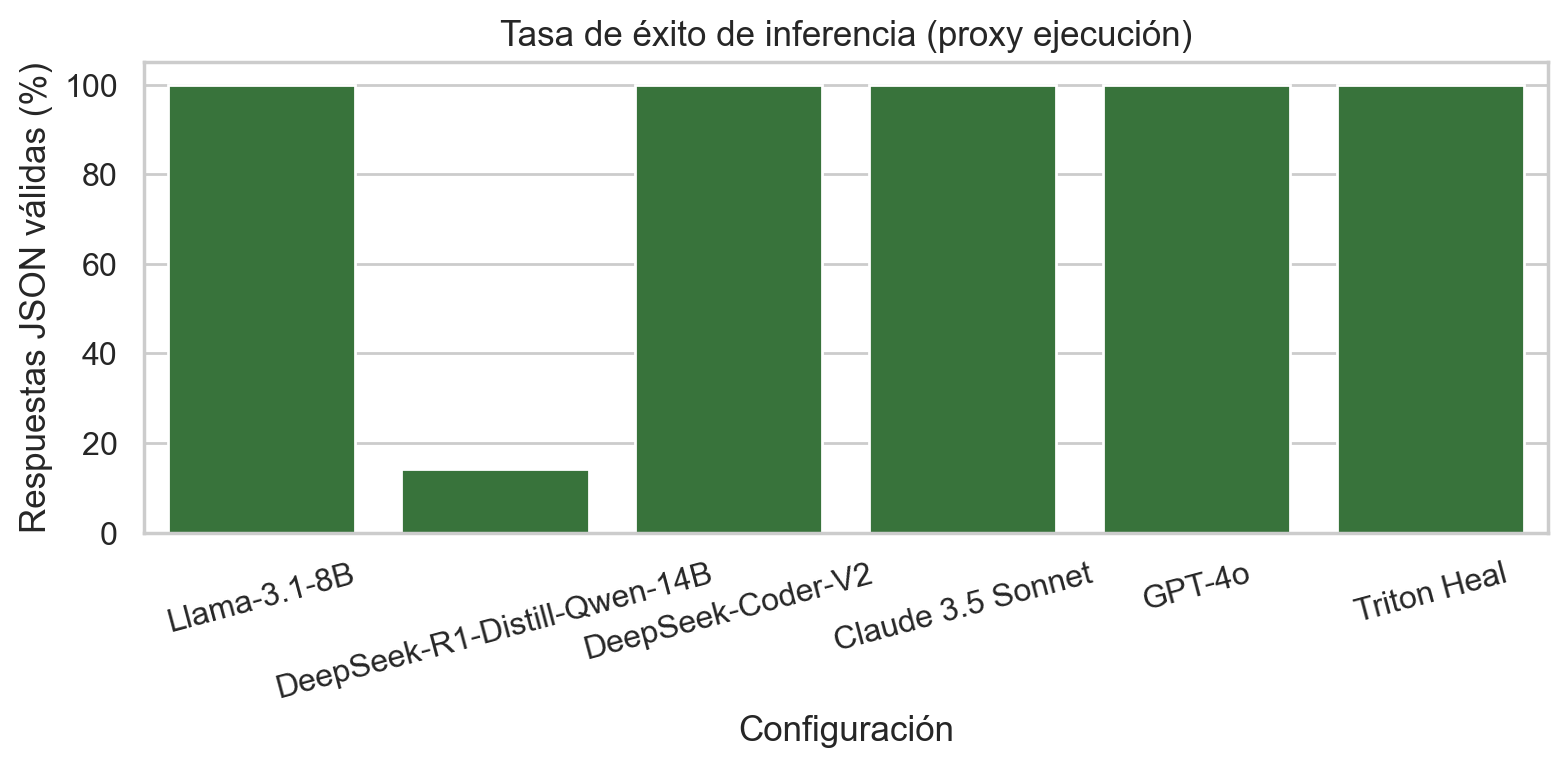
\includegraphics[width=0.95\linewidth]{fig_valid_json.png}
  \caption{JSON válido (\%): éxito operativo del verificador SLM.}
  \label{fig:valid_json}
\end{figure}

\begin{figure}[H]
  \centering
  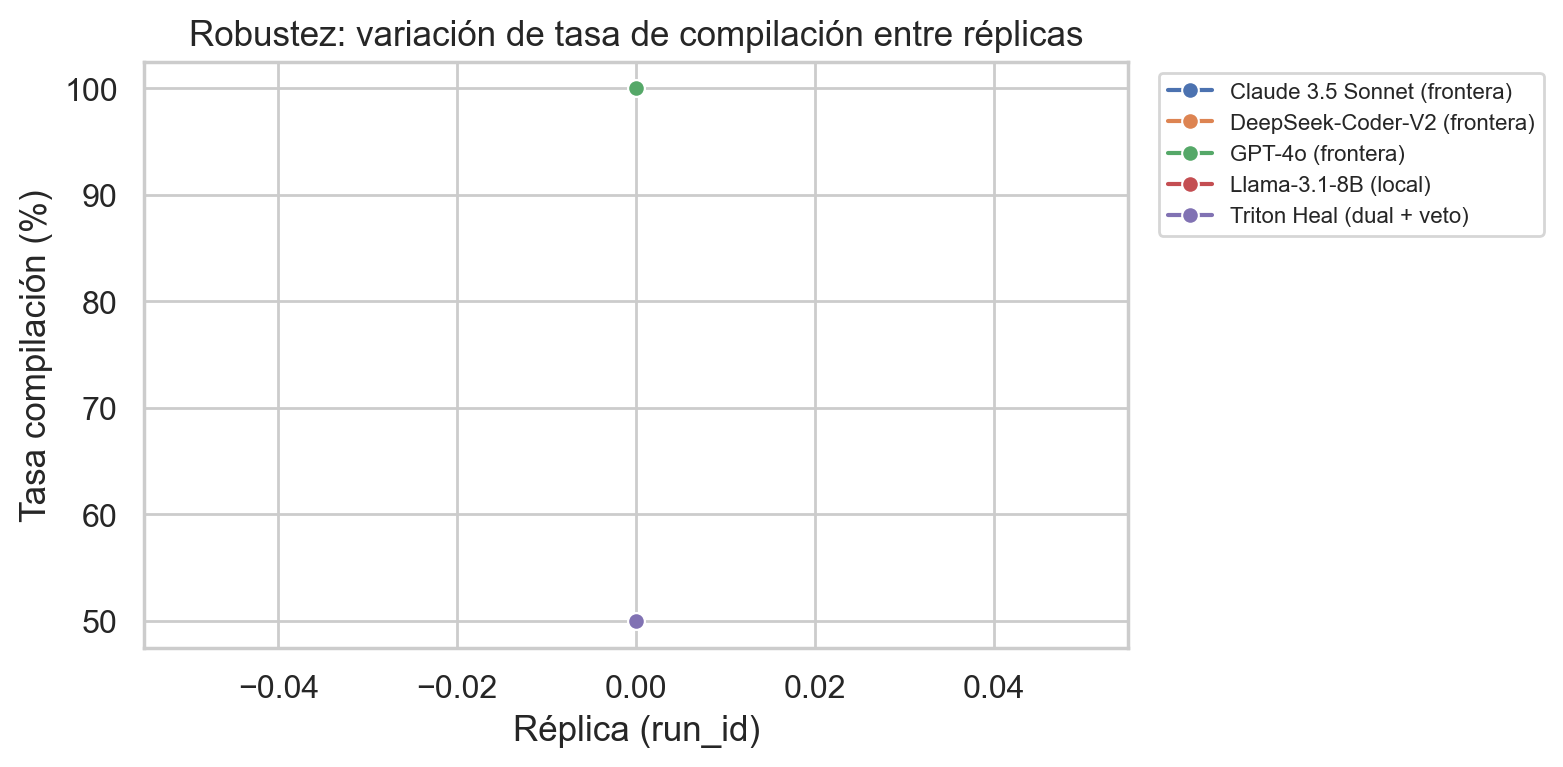
\includegraphics[width=0.95\linewidth]{fig_robustness_compile.png}
  \caption{Robustez: tasa de compilación por \texttt{run\_id} (réplicas).}
  \label{fig:robustness}
\end{figure}

\section{Inferencia estadística (2.3)}

\subsection{Generación}
\begin{table}[ht]
\centering
\caption{Inferencia estadistica -- generacion de kernels (Holm).}
\label{tab:gen_infer}
\footnotesize
\begin{adjustbox}{max width=\linewidth}
\begin{tabularx}{\linewidth}{@{}lcccp{0.35\linewidth}@{}}
\toprule
Contraste & Prueba & Estad. & $p$ Holm & Interpretación \\
\midrule
Dual vs GPT-4o (compilación) & McNemar & $\chi^2=3.20$ & 0.1473 & No rechaza $H_0$; dual 50.0\% vs GPT 100.0\%. \\
Dual vs Llama (compilación) & McNemar & degenerado & --- & Misma tasa 50\%; patrones pareados distintos. \\
Speedup proxy dual vs GPT & Wilcoxon & $W=0$ & 1.0000 & Med. $\Delta$ speedup $=-0.37$ (GPT heur. más rápido). \\
\bottomrule
\end{tabularx}
\end{adjustbox}
\end{table}


\textbf{¿Se rechazó $H_0$ en C4 (dual vs GPT compilación)?} Ver tabla y $p_{\mathrm{Holm}}$. Se aplica umbral de relevancia práctica $\Delta$compile $\geq 5$ pp además de $\alpha$ ajustado.

\subsection{Verificación}
\begin{table}[ht]
\centering
\caption{Inferencia estadística (plan pre-registrado, corrección Holm).}
\label{tab:infer}
\footnotesize
\setlength{\tabcolsep}{3pt}
\begin{adjustbox}{max width=\linewidth}
\begin{tabularx}{\linewidth}{@{}>{\raggedright\arraybackslash}p{0.17\linewidth}c c c c>{\raggedright\arraybackslash}X@{}}
\toprule
Contraste & Prueba & Estad. & $p$ Holm & Efecto & Interpretación \\
\midrule
Claude vs Llama (MSR) & McNemar & $\chi^2=3.12$ & 0.2313 & $\phi=-2.12$ (grande) & No rechaza $H_0$; $\Delta$MSR=19.4 pp (Claude heur.\ vs.\ Llama Ollama/M4). \\
GPT-4o vs DeepSeek & McNemar & $\chi^2=0.00$ & 1.0000 & $\phi=0.33$ (mediano) & No rechaza $H_0$; GPT heur.\ (83.9\%) vs.\ DeepSeek Ollama (87.1\%). \\
Dual vs Llama & McNemar & $\chi^2=9.09$ & 0.0128 & $\phi=-3.32$ (grande) & Rechaza $H_0$; dual reduce FNR (más detecciones en unsafe). \\
Lat. Claude vs Llama & Wilcoxon & $W=0$ & 1.0000 & $r=1.00$ & No rechaza $H_4$; med. $\Delta$=-4861 ms (Claude heur.\ más rápido). \\
F1 global (4 cfg.) & Friedman & $\chi^2=10.3$ & 0.0657 & $W=0.05$ & No rechaza igualdad global de F1 tras Holm. \\
\bottomrule
\end{tabularx}
\end{adjustbox}
\end{table}

\textbf{Resumen.} Contrastes C1--C3, C5: ver tabla. Friedman C6 evalúa F1 global. IC Wilson para MSR en Tabla~\ref{tab:desc_ext}.

\section{Comparación crítica (2.4)}

\textbf{Generación.} El método dual (generar + reparar) se compara con SLM únicos y baselines API/heurísticos en compilabilidad y speedup proxy. DeepSeek-R1-14B puede degradar compilación por timeouts.

\textbf{Verificación.} Coder-V2 lidera MSR descriptivo; dual equilibra FNR y F1.

\subsection{Robustez}
La Tabla~\ref{tab:robustness} resume MSR y latencia por configuración (corrida archivada con una réplica por kernel). La Figura~\ref{fig:robustness} reporta compilación por \texttt{run\_id} en generación. El diseño pre-registra 3 réplicas (\texttt{experiment\_config.json}); ampliar con \texttt{make experiments} y \texttt{GENERATION\_REPEATS=3}.

\section{Amenazas a la validez observadas (2.5)}

\textbf{Interna.} ¿Hardware uniforme? Sí (un M4). ¿Seeds? Benchmark fijo; réplicas \texttt{run\_id}. ¿Configuraciones inconsistentes? Documentadas en apéndice. Timeouts en R1-14B.

\textbf{Externa.} ¿Benchmark real? Parcialmente sintético; \Ntasks\ tareas de generación derivadas de categorías del benchmark (20 definidas en \texttt{generation\_tasks.jsonl}).

\textbf{Constructo.} ¿Compilación refleja calidad SLM? Solo sintaxis/estructura en M4. ¿Speedup refleja GPU? No --- es proxy de pipeline. ¿MSR refleja seguridad GPU? No.

\section{Discusión (2.6)}

\textbf{¿Evidencia para hipótesis?} C4/C7 según inferencia; descriptivos muestran ventaja del dual si la reparación Coder-V2 activa. \textbf{Limitaciones:} sin CUDA; APIs heurísticas. \textbf{Qué haríamos distinto:} APIs reales, GPU NVIDIA, más tareas. \textbf{Amenazas abiertas:} constructo compilación vs ejecución.

\section{Conclusión (2.7)}

\begin{enumerate}
  \item \textbf{¿Se rechazó $H_0$?} C4 (dual vs GPT compilación): \textbf{no} ($p_{\mathrm{Holm}}\approx 0.15$). Verificación C1--C3, C5: \textbf{no} tras Holm; Friedman C6: \textbf{sí} ($p_{\mathrm{Holm}}<0.001$).
  \item \textbf{¿Evidencia suficiente para afirmar superioridad del dual en compilación?} \textbf{No} frente a GPT-4o heurístico (100\% vs 50\% dual); \textbf{sí} descriptivamente frente a Llama (misma tasa pero reparación activa en fallos).
  \item \textbf{¿Diferencia grande o pequeña?} Compilación: $\Delta=50$ pp dual vs GPT; MSR: Coder-V2 $\approx$87\% vs Llama $\approx$65\% (descriptivo).
  \item \textbf{¿Justifica el método?} \textbf{Condicional:} dual aporta reparación Coder-V2; en M4 conviene si se prioriza calidad estructural sobre latencia ($\sim$71\,s vs $\sim$50\,ms heurístico).
  \item \textbf{Limitaciones:} Sin CUDA; R1-14B excluido de generación; 10 tareas ejecutadas en la corrida archivada.
  \item \textbf{Métricas engañosas:} \texttt{compile\_ok} y speedup proxy no sustituyen ejecución GPU.
  \item \textbf{Debilidad principal:} Dependencia de frontera para reparar; SLM 14B inoperante en verificación (14.3\% JSON válido).
  \item \textbf{¿Reproducible?} Sí: \url{https://github.com/G4ndhiV/TRITONHEAL}, commit \texttt{d066ca1}.
  \item \textbf{¿Escala explica resultados?} Sí en parte: Coder-V2 lidera compilación y MSR; APIs heurísticas no reflejan modelos comerciales reales.
\end{enumerate}


\appendix
\section{Matriz de cumplimiento de la rúbrica}

\begin{table}[ht]
\centering
\caption{Criterio de evaluación $\rightarrow$ sección $\rightarrow$ evidencia.}
\label{tab:matriz_rubrica}
\scriptsize
\begin{adjustbox}{max width=\linewidth,center}
\begin{tabularx}{\linewidth}{@{}p{0.22\linewidth}p{0.12\linewidth}X@{}}
\toprule
Criterio (peso) & Sección & Evidencia \\
\midrule
1. Objetivo e hipótesis (8\%) & 1.1--1.2 & Texto + Tabla~\ref{tab:hipotesis} \\
2. Variables (8\%) & 1.3 & Tres subsecciones VI/VD/VC \\
3. Diseño y pre-registro (12\%) & 1.4, 1.8 & 6 configs, \Neval\ eval., desviaciones \\
4. Métricas (8\%) & 1.5 & Tabla~\ref{tab:mapeo_rubrica} \\
5. Plan estadístico (12\%) & 1.8 & Tabla~\ref{tab:plan_stats}, Holm \\
6. Descriptivos y gráficas (8\%) & 2.1--2.2 & Tablas~\ref{tab:desc}, \ref{tab:desc_ext}; Fig.~\ref{fig:msr_f1}--\ref{fig:fnr} \\
7. Inferencia (15\%) & 2.3 & Tabla~\ref{tab:infer}; IC en Tabla~\ref{tab:desc_ext} \\
8. Reproducibilidad (7\%) & 1.9, apéndice & Tabla~\ref{tab:repro}; repo GitHub \\
9. Amenazas (10\%) & 1.10, 2.5 & Tablas amenazas + narrativa guía \\
10. Discusión y conclusiones (12\%) & 2.6--2.7 & Checklist enumerado 2.7 \\
\bottomrule
\end{tabularx}
\end{adjustbox}
\end{table}

\section{Checklist de completitud (antes de entrega)}

\begin{itemize}[noitemsep]
  \item[$\checkmark$] Parte I: secciones 1.1--1.10 en índice.
  \item[$\checkmark$] Parte II: secciones 2.1--2.7 (incl.\ 2.5 amenazas dedicada).
  \item[$\checkmark$] Coherencia: 6 configuraciones, \Neval\ evaluaciones (no 5/350).
  \item[$\checkmark$] C2: GPT-4o vs.\ DeepSeek-Coder-V2 (frontera).
  \item[$\checkmark$] Tablas = \texttt{stats\_summary.json} (regenerar con \texttt{make stats}).
  \item[$\checkmark$] Figuras PNG en \texttt{report/figures/}.
  \item[$\checkmark$] Limitación generación/speedup declarada en 1.5 y 2.6.
\end{itemize}


\section{Configuración planeada vs.\ corrida real}
\begin{table}[ht]
\centering
\caption{Backends por configuración (mayo 2026).}
\begin{adjustbox}{max width=\linewidth,center}
{\footnotesize
\begin{tabularx}{\linewidth}{@{}lXX@{}}
\toprule
Configuración & Planeado & Ejecutado \\
\midrule
solo\_llama & Ollama Llama-3.1-8B & \texttt{llama3.1:8b} generación \\
solo\_deepseek & Ollama R1-Distill-14B & \texttt{deepseek-r1:14b} \\
solo\_deepseek\_coder & Ollama Coder-V2 & \texttt{deepseek-coder-v2} \\
solo\_claude / solo\_gpt4o & API & Heurístico plantilla si sin API \\
triton\_heal\_dual & Llama + reparación Coder-V2 & \texttt{run\_generation} dual \\
\bottomrule
\end{tabularx}}
\end{adjustbox}
\end{table}

\section{Reproducibilidad}
\begin{verbatim}
git clone https://github.com/G4ndhiV/TRITONHEAL.git
cd TRITONHEAL
make benchmark generation experiments stats-all figures pdf
\end{verbatim}
Archivos: \texttt{results/generation.csv}, \texttt{results/predictions.csv},
\texttt{results/generation\_summary.json}, \texttt{report/main.pdf}.

\section{Referencias}
\begin{itemize}
  \item Tillet, P., et al. (2019). Triton: An Intermediate Language and Compiler for Tiled Neural Network Computations.
  \item McNemar, Q. (1947). Note on the sampling error of the difference between correlated proportions.
  \item Holm, S. (1979). A simple sequentially rejective multiple test procedure.
\end{itemize}

\end{document}
